\StartPlate{V28}{The even-order negative control}{A nonzero cocycle survives when every permitted coboundary vanishes.}
\begin{center}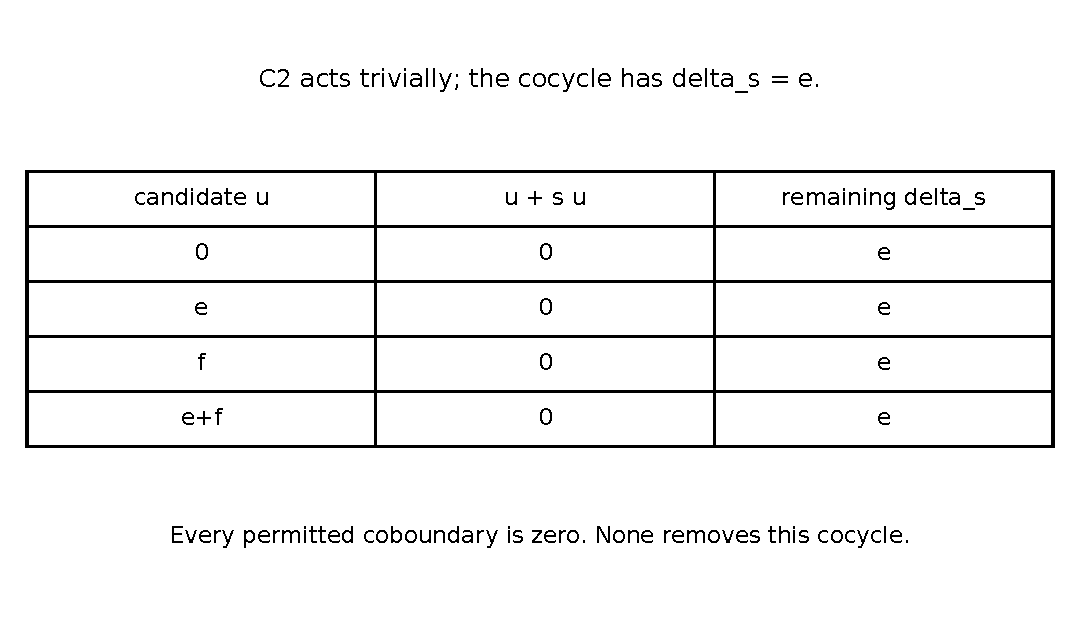
\includegraphics[width=\linewidth]{figures/V28.pdf}\end{center}
Let $C_2=\{1,s\}$ act trivially on the nonzero module $A=\F_2^2$. The assignment $\delta_1=0$, $\delta_s=e$ satisfies the cocycle equation, since $e+e=0$. For every proposed correction $u$,
\[
u+su=u+u=0,
\qquad u+\delta_s+su=e.
\]
The four rows exhaust the module. None removes the discrepancy. Thus the odd-order hypothesis of the preceding plate is mathematically active.

This does not say that every even-order action problem is obstructed. It supplies one exact counterexample to an unrestricted averaging claim. Other actions and cocycles may admit corrections. In the arithmetic problem, it remains necessary to compute the actual discrepancy and respect the permitted transformations. Declaring every projective or equivariance mismatch removable would erase precisely the information this example retains.
\vfill\PlateSource{Exact obstruction model}{Part III, Section 29.2}{74}
